O algoritmo \algname{Parallel U-Curve Search (PUCS)} foi desenvolvido 
para resolver o problema U-Curve particionando o espaço de busca em 
partes que podem ser resolvidas independentemente e de forma paralela. 
Além disso, a dinâmica desse algoritmo depende de parâmetros que 
determinam o tempo de execução e qualidade da solução obtida, permitindo
ao usuário adequar o algoritmo aos recursos computacionais disponíveis. 

\section{Princípios do algoritmo}
 
\subsection{Partição do espaço de busca}
Seja $S$ o conjunto de características do problema em questão. O 
primeiro passo do particionamento é escolher arbitrariamente $S'$ um 
subconjunto de $S$; de maneira complementar, definimos 
$\overline{S'} = S \setminus S'$. Agora, sejam $X, Y \in \powerset (S)$
e $\sim$ a relação:

\begin{equation*}
    X \sim Y \iff (X \cap S') = (Y \cap S')
\end{equation*}
Esta relação é de equivalência, pois nela valem:

\begin{itemize}
    \item{reflexividade}
        \begin{align*} 
            X \sim X \text{, pois }
            (X \cap S') = (X \cap S')
        \end{align*} 
    \item{simetria}
        \begin{align*}
            X \sim Y  & \iff \\
            (X \cap S') = (Y \cap S') & \iff \\
            (Y \cap S') = (X \cap S') & \iff \\
            Y \sim X 
        \end{align*}
    \item{transitividade,}
        \begin{align*}
            X \sim Y, Y \sim Z & \Rightarrow \\
            (X \cap S') = (Y \cap S') = (Z \cap S') & \Rightarrow \\
            (X \cap S') = (Z \cap S') & \Rightarrow \\
            X \sim Z
        \end{align*}
\end{itemize}
Portanto, o conjunto das classes de equivalência definidas por $\sim$ é
uma partição do espaço de busca original. Tome como exemplo o conjunto
$S = \{a, b, c\}$; se $S' = {a}$, então existem duas classes de 
equivalência no particionamento do espaço de busca que definimos, 
formados pelos conjuntos $\{\emptyset, b, c, bc\}$ e $\{a, ab, ac, 
abc\}$.

Pela definição da relação $\sim$ temos que a presença de cada 
característica de $S'$ em uma dada parte do reticulado não muda, isto é,
ou ela está presente em todos subconjuntos da parte ou não está presente
em nenhum, portanto, dizemos que estas variáveis são {\bf fixas}. De 
modo análogo, as variáveis de $\overline{S'}$ são {\bf livres}. Tanto 
variáveis fixas quanto livres podem definir reticulados Booleanos junto 
a relação de ordem parcial $\subseteq$.

O conjunto $\powerset (S')$ induz um reticulado Booleano em que cada
elemento representa uma classe de equivalência do espaço de soluções
do problema original, chamamos este de {\bf reticulado externo}. Para 
cada classe de equivalência (nó do reticulado externo), o conjunto 
$\powerset (\overline {S'})$ induz um outro reticulado Booleano ({\bf
reticulado interno}) em que cada elemento representa um subconjunto de
problema original. Seja $A \in \powerset (S')$ um elemento do reticulado 
externo, então cada $B \in \powerset (\overline{S'})$ do reticulado 
interno em $A$ representa o conjunto $X = B \cup A$ do espaço de busca
do problema original. A figura \ref{fig:pucs_parts} apresenta um exemplo
de particionamento feito pelo \algname{PUCS} em um reticulado Booleano
com cinco características.

\begin{figure}[!ht]
  \centering 
  \begin{tabular}{c c}
    \subfigure[] {\scalebox{0.4}{
     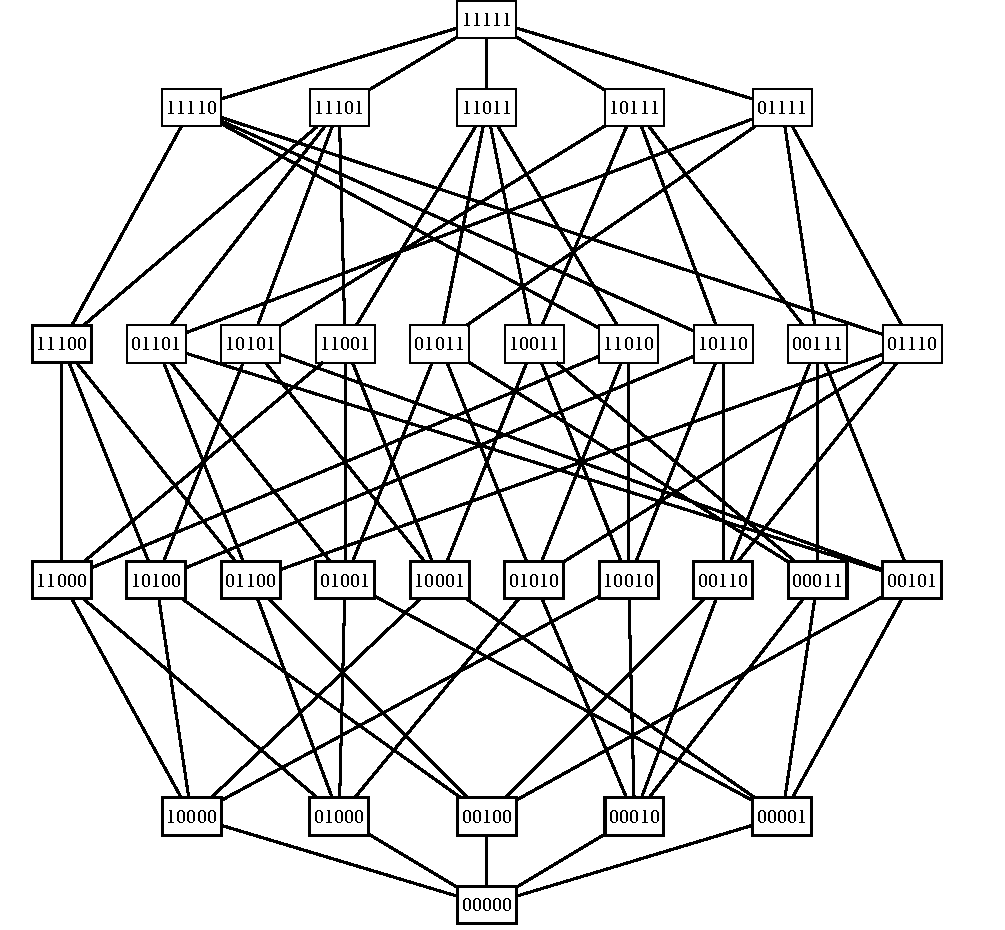
\includegraphics[clip=true]{pucs/partition/full_lattice.pdf}}
     \label{fig:pucs_part:full} }
    & 
    \subfigure[] {\scalebox{1}{
    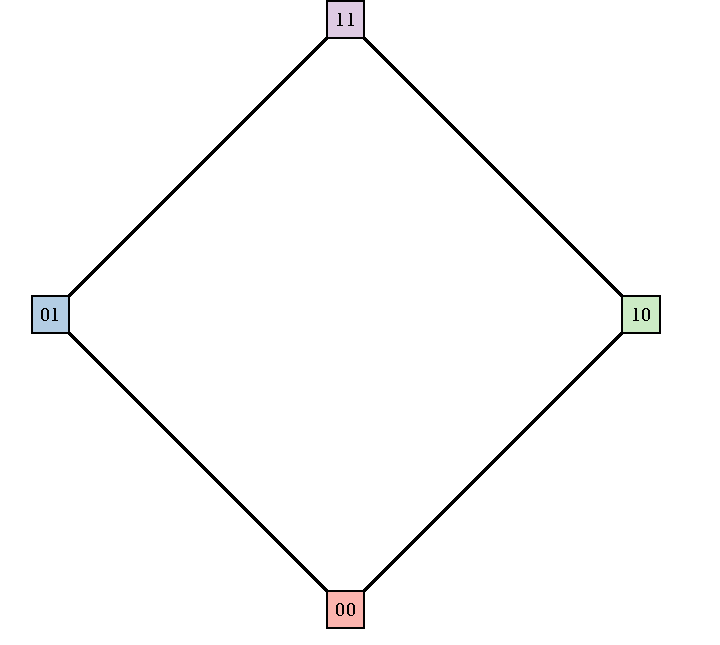
\includegraphics[clip=true]{pucs/partition/external_lattice.pdf}}
    \label{fig:pucs_part:external} }
    \\
    \subfigure[] {\scalebox{1}{
    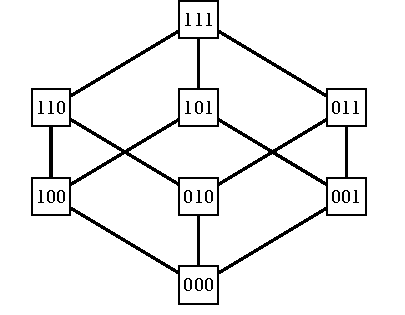
\includegraphics[clip=true]{pucs/partition/internal_lattice.pdf}}
    \label{fig:pucs_part:internal} }
    &
    \subfigure[] {\scalebox{0.4}{
    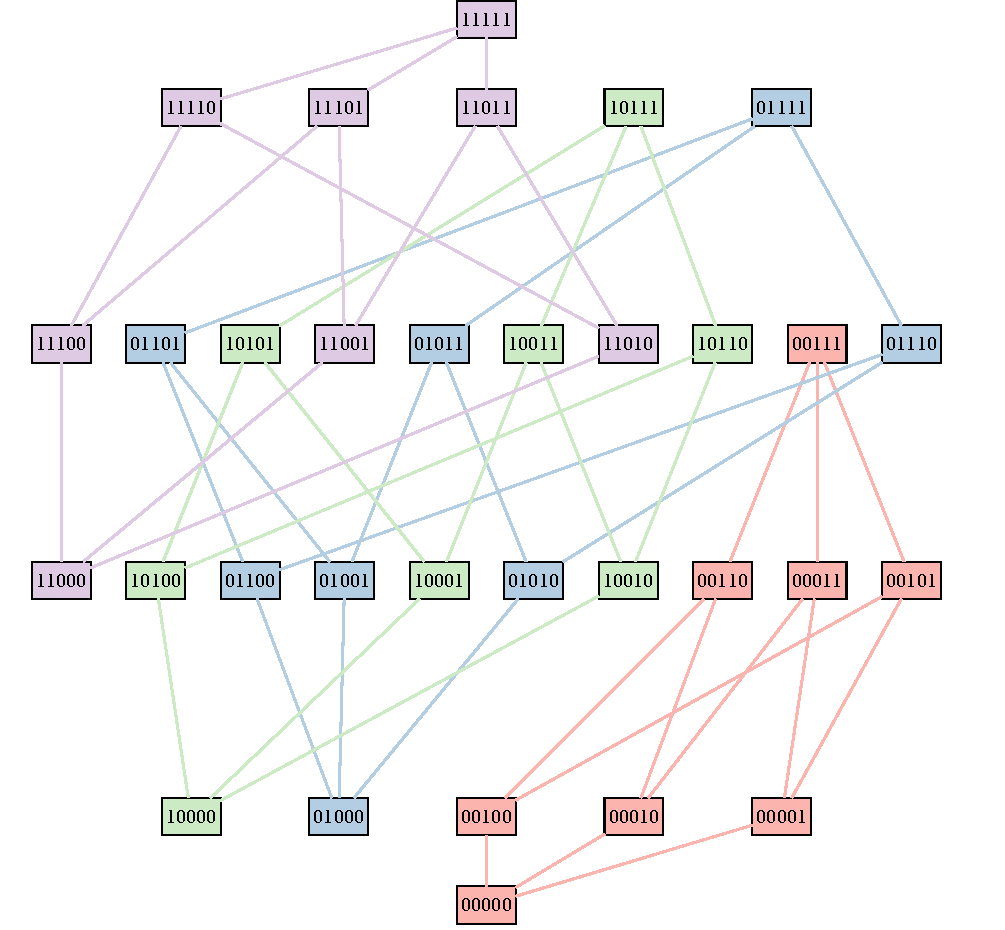
\includegraphics[clip=true]{pucs/partition/all_parts.pdf}}
    \label{fig:pucs_part:parts} }   
    \\
  \end{tabular}
    \caption{Exemplo de particionamento feito pelo algoritmo 
    \algname{PUCS} em uma instância com cinco características; o 
    reticulado Booleano desta instância é representado na figura 
    \ref{fig:pucs_part:full}. Neste particionamento, as duas primeiras
    variáveis formam o conjunto de variáveis fixadas, definindo o 
    reticulado externo (figura \ref{fig:pucs_part:external}) enquanto 
    as outras três definem os reticulados internos, que são cópias do
    reticulado da figura \ref{fig:pucs_part:internal}. A figura 
    \ref{fig:pucs_part:parts} mostra o reticulado Booleano original, sem
    as arestas que ligam duas partes diferentes, e a cor de cada nó 
    representa a qual parte tal nó pertence, de acordo com as cores
    do reticulado externo em \ref{fig:pucs_part:external}
    Note que, de fato, 
    cada parte forma um reticulado pequeno de mesmo tamanho e com mesma 
    estrutura que o reticulado da figura \ref{fig:pucs_part:internal}}
  \label{fig:pucs_parts} 
\end{figure}

Os reticulados internos e externo elucidam a estrutura recursiva do 
problema de seleção de características e sugerem que podemos construir 
uma solução ao problema original a partir de soluções de outros 
problemas, sobre os reticulados externo e internos, abordagem conhecida
em computação como divisão e conquista. Seja $\langle S, c \rangle$ uma 
instância do problema de seleção de características, $S'$ o conjunto de 
variáveis fixas, $\overline{S'}$ o conjunto de variáveis livres, e 
$A \in \powerset (S')$ um subconjunto que é nó do reticulado externo, 
então podemos definir um outro problema de seleção de características 
$\langle \overline{S'}, c_{A} \rangle$ em que 
\begin{align*}
    c_{A} (X) = c (X \cup A).
\end{align*}
Resolver a instância $\langle \overline{S'}, c_{A} \rangle$ é 
essencialmente achar o mínimo do problema inicial restrito a classe de
equivalência de $A$, dizemos também que estamos resolvendo a parte $A$. 
Se soubermos em qual classe o mínimo global reside, podemos resolver 
apenas tal parte e garantir que a solução encontrada é a solução do 
problema original.

O algoritmo \algname{PUCS} percorre o reticulado externo recolhendo 
partes candidatas a conter o mínimo e resolve cada uma destas, 
escolhendo o mínimo das soluções destas partes como o mínimo global do 
problema.


\subsection{Dinâmica do algoritmo}
Para escolher partes candidatas a conter o mínimo global do problema,
o algoritmo \algname{PUCS} faz um passeio aleatório no reticulado 
externo. O algoritmo se inicia escolhendo arbitrariamente um nó inicial 
que pertence ao espaço de busca, então a cada passo as condições de podas
são verificadas e escolhe-se aleatoriamente um vizinho do nó corrente
que ainda pertence ao espaço de busca para se tornar o novo nó corrente.
O algoritmo repete estes passos até que todos os nós do reticulado 
externo tenham sido ou podados ou visitados.

As podas eliminam do reticulado externo intervalos da forma 
$[X, \powerset(S')]$ ou $[\emptyset, X]$ e são realizadas sempre que a 
hipótese de curva em u implica que todas as partes contidas nestes 
intervalos não contém o mínimo global. Para entender o critério de poda,
vamos definir que a {\bf ponta superior} de um reticulado Booleano 
$\powerset (A)$ é o próprio conjunto $A$ e a {\bf ponta inferior} deste
reticulado é o conjunto vazio. Note que no reticulado interno de uma
parte $P$ a ponta inferior representa o próprio conjunto de 
características $P$, enquanto que a ponta superior representa o conjunto
de características $P \cup \overline{S'}$.

\begin{mytheorem}[Critério de poda para o reticulado externo do 
algoritmo \algname{PUCS}]
Sejam $S$ um conjunto de características e $S'$ um conjunto de variáveis
fixas no particionamento definido pelo algoritmo \algname{PUCS}. Dados
$P, Q \in \powerset (S')$ dois elementos do reticulado externo com 
$Q \subseteq P$; se a ponta inferior do reticulado interno de $P$ tem 
custo maior do que a ponta inferior do reticulado interno de $Q$, então 
todas as partes do intervalo $[P, \powerset (S')]$ tem apenas conjuntos 
de características com custo maior do que o custo da ponta inferior de 
$Q$.
\end{mytheorem}
\begin{proof}
Se o custo da ponta inferior do reticulado interno de $P$ é maior do que
a de $Q$, então:
\begin{align*}
    c_Q (\emptyset) < c_P (\emptyset) & \text{, portanto} \\
    c (\emptyset \cup Q) < c (\emptyset \cup P) &\\
    c (Q) < c (P)
\end{align*}
Como $Q \subseteq P$, temos que existe uma cadeia que passa pelas pontas
inferiores de $Q$ e $P$. Além disso, para qualquer conjunto de 
características $X \in \powerset (S)$, com $P \subseteq X$, a hipótese 
de curva em U garante que:
\begin{align*}
    c (P) \leq max \{c (Q), c (X)\}
\end{align*}
e $c (P) > c (Q)$ implica que $c (X) \geq c (P)$, isto é, qualquer 
elemento do reticulado Booleano original que cobre a ponta inferior de 
$P$ tem custo estritamente maior do que o custo da ponta inferior de $Q$.
Note que para qualquer parte $R$ do intervalo $[P, \powerset (S')]$, 
vale que $P \subseteq R$, e como a ponta inferior de $P$ não contém 
nenhum elemento de $\overline {S'}$, então qualquer conjunto de 
características da parte $R$ cobre a ponta inferior de $P$ e portanto 
tem custo estritamente maior do que o custo da ponta inferior da parte 
$Q$.
\end{proof}

% TODO: escrever o critério dual
